\documentclass{article}

\usepackage{Vor2018skil}

\title{Tölvunarfræði 2, \semester \\ Námsáætlun og upplýsingar}
\author{}

\begin{document}
\maketitle
\hypersetup{pdftitle={Tölvunarfræði 2 - \semester}}

\section{Námsáætlun}
\label{sec:schedule}

Námskeiðið er tvískipt. 

Fyrri hluti námskeiðsins er þrjár vikur. Í þeim hluta verður farið í grundvallaratriði forritunarmálsins C++.

Aðalviðfangsefni námskeiðsins, gagnagrindur og reiknirit sem á þeim vinna, koma fyrir í seinni hluta. Forritun í Java og C++ kemur við sögu. Seinni hluti spannar afgang kennslumisserisins, samtals 11 vikur.

Námskeiðið er framhaldsnámskeið Tölvunarfræði 1, gert er ráð fyrir að efni þess námskeiðs sé á hreinu. Nemendur án bakgrunns í Java eða C++ munu þurfa að kynna sér grunnatriði þessara forritunarmála upp á eigin spýtur.

\begin{table}
\caption{Námsáætlun eftir vikum}
\label{tab:schedule}
\begin{center}
\renewcommand{\arraystretch}{1.2}
\begin{tabularx}{\linewidth}{lcXp{1cm}}
\toprule
Vika&Dagsetning&Námsefni&Kafli\\
\midrule
1	&12/1	& Kynning á námskeiðinu, kynning á C++ &C++ 1\\
2	&19/1	& Minnisuppbygging í C++, Hlutbundin forritun í C++&C++ 2\\
3	&20/1	& Meira um hlutbundna forritun, kynning á STL&C++ 3\\
4	&26/9	& Þýðing forrita, uppbygging forrita, forritun í Java, tögun&Alg 1\\
5	&2/2	& Skjóður, biðraðir, hlaðar, greining reiknirita&Alg 1\\
6	&9/2	& Röðunarreiknirit&Alg 2\\
7	&16/2	& Röðunarreiknirit, forgangsbiðraðir&Alg 2\\
8	&23/2	& Leit, leitartré&Alg 3\\
9	&2/3	& Leitartré, hakkatöflur&Alg 3\\
10	&9/3	& Net, stefnd net&Alg 4\\
11	&16/3	& Minnstu spanntré, stystu vegir&Alg 4\\
12	&23/3	& Strengir, trie&Alg 5\\
13	&30/3	& Páskaleyfi&-\\
14	&6/4	& Strengjaleit, reglulegar segðir&Alg 5\\
15	&13/4	& Skekkjumörk í námsáætlun&-\\
16	&20/4	& Skekkjumörk í námsáætlun&-\\
\bottomrule
\end{tabularx}
\end{center}
\end{table}

\section{Kennari}
Aðalkennari er Eiríkur Ernir Þorsteinsson. Aðsetur er í Tæknigarði, 2. hæð, stofa 214. Sjá mynd \ref{fig:taeknigardur}.

Til að hafa samband við kennara er ráðlagt að setja inn þráð á \href{https://piazza.com/hi.is/spring2018/tl203g}{Piazza}. Allar fyrirspurnir sem ekki fela í sér persónulegar upplýsingar ættu að fara þangað. 

Tölvupóstfang er \href{mailto:ernir@hi.is}{ernir@hi.is}.

\begin{figure}
\caption{Önnur hæð í Tæknigarði. Kennara má finna í stofu 212.}
\label{fig:taeknigardur}
\begin{center}
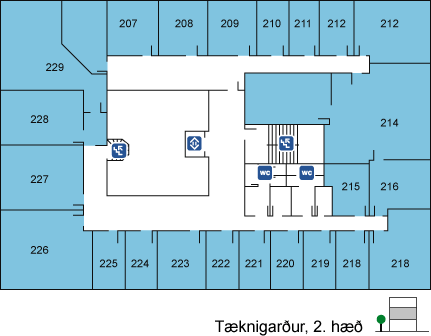
\includegraphics[width=0.5\linewidth]{taeknigardur}
\end{center}
\end{figure}

\section{Tímar og námstilhögun}
Aðalkennsla fer fram í vikulegum fyrirlestri. Dæmatímar eru á mánudögum og þriðjudögum. Tímasetningar og staðsetningar má sjá í Uglu.

\subsection{Mætingaskylda}
Ekki er skylda að mæta í fyrirlestra eða dæmatíma. Leyfilegt er að mæta í núll eða fleiri dæmatíma eftir því sem þörf er á. Nemendur eru ábyrgir fyrir því að forgangsraða tíma sínum.

\subsection{Upptökur á fyrirlestrum}
Fyrirlestrar eru teknir upp þegar tæknin leyfir. Varað er við því að treysta á upptökur í stað mætingar í fyrirlestra.

\section{Námsbækur}
Aðalkennslubók er \emph{Algorithms}, fjórða útgáfa, eftir Sedgewick og Wayne. Kennsla eftir þeirri bók hefst í fjórðu kennsluviku, eftir kynningu á C++ (sjá \nameref{tab:schedule}). 

Til stuðnings við er bent á \emph{C++ in One Hour a Day}, 8. útgáfa, eftir Siddhartha Rao. Litið verður til hennar við yfirferð á C++, en ekki verður vísað beint í bókina.

\begin{figure}
    \caption{Kennslubækur}
    \begin{multicols}{2}
    \begin{center}
    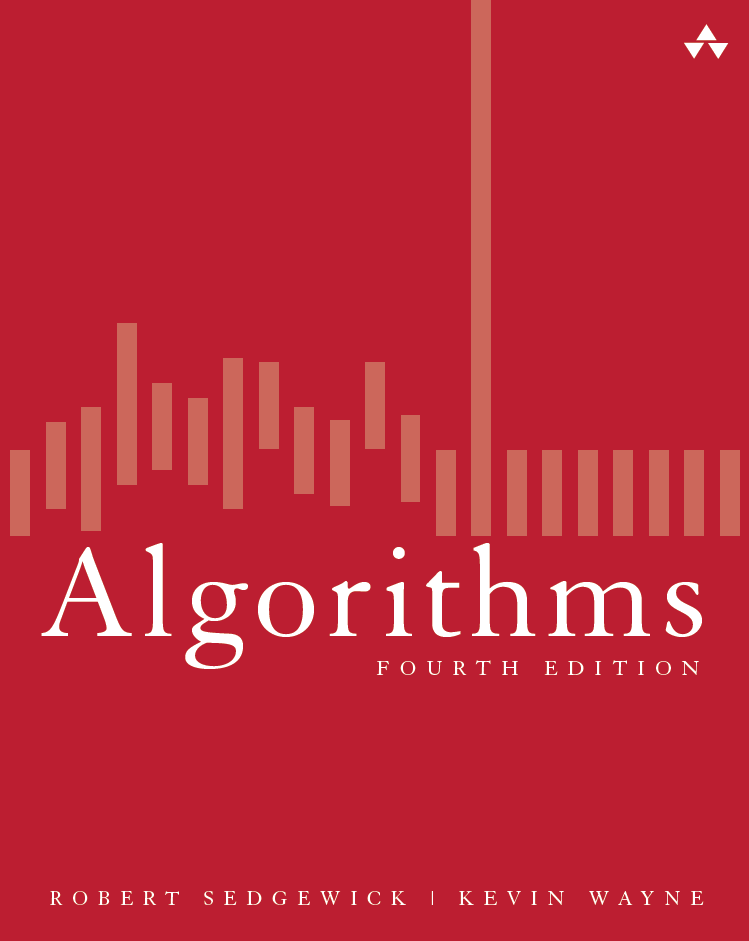
\includegraphics[height=8cm]{algorithms4th}
    \end{center}
    
    \begin{center}
    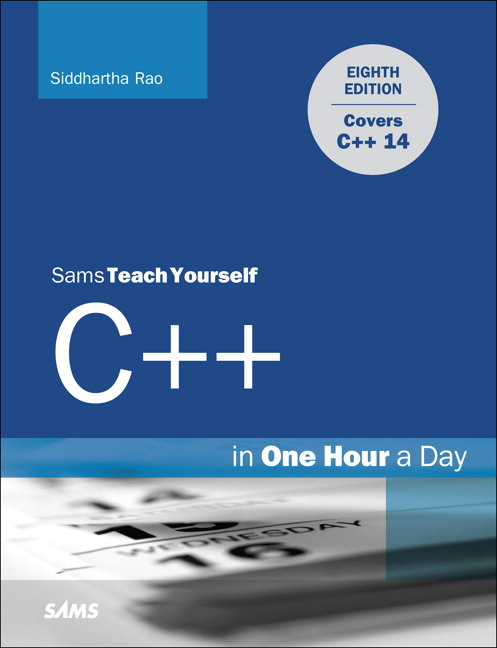
\includegraphics[height=8cm]{teachyourself}
    \end{center}
    \end{multicols}
\end{figure}

\newpage
\section{Námsmat, einkunnir og próf}
\subsection{Skilaverkefni}
Vikuleg verkefnaskil eru í námskeiðinu. Meðaleinkunn 10 bestu skilaverkefnanna er 50\% af lokaeinkunn. 

Verkefnunum skal skila á Gradescope.com (sjá \nameref{sec:tools}). \emph{Ekki er tekið við seinum skilum. Vönduð framsetning á verkefnunum skiptir máli og gildir til einkunnar.}

Nauðsynlegt er að skila fjórum af fyrstu sex skilaverkefnunum til að öðlast próftökurétt. Þessi fyrstu sex skilaverkefni verða einstaklingsverkefni, seinni verkefnum má skila í pörum.

\subsubsection{Lausnir á skilaverkefnum}

Í hverri viku munu dæmatímakennarar velja eina eða fleiri góðar lausnir frá nemendum til að birta öllum.

Vilji nemandi ekki að lausn sín sé birt þrátt fyrir að hún sé góð eða að hún sé eingöngu birt undir nafnleynd skal slíkt tekið fram í svari við hverri spurningu um sig.

\subsection{Próf og lokaeinkunn}
Vægi lokaprófs er 50\% af lokaeinkunn. Ekki er miðmisserispróf í námskeiðinu.

Lágmarkseinkunn er 5. Nauðsynlegt er að ná lágmarkseinkunn á lokaprófi sem og í námskeiðinu sem heild til að standast námskeiðið. Lokaeinkunn verður námunduð að heilum aukastaf.

\section{Kennslutól}
\label{sec:tools}
Vefkennslutól verða notað eftir föngum. Mælt er með að nemendur skrái sig inn á eftirfarandi þjónustur sem allra fyrst:
\begin{itemize}
 \item \href{https://piazza.com/hi.is/spring2018/tl203g}{Piazza} er fyrirspurnavefurinn sem notaður er í námskeiðinu. Skráningin í námskeiðið á að vera sjálfvirk, en hafi það misfarist á að vera hægt að skrá sig handvirkt. Allar spurningar sem snúa að námskeiðinu ættu að fara inn á Piazza frekar en í tölvupóst.
 \item \href{https://gradescope.com/courses/14122}{Gradescope.com} er vefkerfið sem notað er til að taka við skilaverkefnum. Nemendur þurfa að skrá sig sjálfir á þennan vef. Aðgangskóði námskeiðsins er \texttt{MZR4DK}. Mikilvægt er að skrá sig á Gradescope með fullu nafni (íslenskir stafir eru leyfilegir) og með því að nota HÍ-netfang. Kerfið tekur við \texttt{.pdf} skrám.
\end{itemize}
Fyrir utan vefkennslutól er nauðsynlegt að nemendur setji upp þýðendur fyrir C++ og Java ásamt viðeigandi ritlum á eigin tölvum eða útvegi sér aðgang að slíkri vél.

\section{Undanþágur og sérúrræði}

Ef þörf er á sérstökum úrræðum eða undanþágum skal hafa samband við \href{http://nshi.hi.is/}{Náms- og starfsráðgjöf HÍ}\footnote{\url{nshi.hi.is}}. Hægt er að leita til hennar með öll persónuleg mál sem snúa að náminu.

\vfill

\includegraphics[width=0.5\linewidth]{hi-von-logo}
\end{document}